\documentclass[conference]{IEEEtran}
\IEEEoverridecommandlockouts
% The preceding line is only needed to identify funding in the first footnote. If that is unneeded, please comment it out.
\usepackage{cite}
\usepackage{amsmath,amssymb,amsfonts}
\usepackage{algorithmic}
\usepackage{graphicx}
\usepackage{textcomp}
\usepackage{xcolor}
\usepackage{url}
\usepackage{soul}
\usepackage{multirow}
\usepackage{lmodern}
\usepackage{framed}
\usepackage{color}
\usepackage{booktabs}
\usepackage{anyfontsize}

\def\BibTeX{{\rm B\kern-.05em{\sc i\kern-.025em b}\kern-.08em
    T\kern-.1667em\lower.7ex\hbox{E}\kern-.125emX}}
\begin{document}
\nocite{*}

\title{Linking Team-level and Organization-level Governance in MLOps through XAI and RAI Connector  \\
% {\footnotesize \textsuperscript{*}Note: Sub-titles are not captured in Xplore and
% should not be used}
% \thanks{Identify applicable funding agency here. If none, delete this.}
}

\author{
\IEEEauthorblockN{Elie Neghawi}
\IEEEauthorblockA{\textit{Electrical and Computer Engineering} \\
\textit{Concordia University}\\
Montreal, Canada \\
e\_negh@encs.concordia.ca}

\and

\IEEEauthorblockN{Yan Liu}
\IEEEauthorblockA{\textit{Electrical and Computer Engineering} \\
\textit{Concordia University}\\
Montreal, Canada \\
yan.liu@concordia.ca}
}

\maketitle

\begin{abstract}
	Adoption of AI systems has been widely used across multiple industry domains at an alerting rate without the focus on it's ethical concerns. To address those concerns, there are an increase number of AI ethics frameworks that have been suggested recently that focus on the algorithmic level rather on the systems level. Nonetheless, some of the system level approaches developed mostly cover a single level governance pattern of the system components in the entire software design lifecycle. However, the need to go beyond the single level  system design AI ethics frameworks to allow not only a better responsible-AI-by-design, but also a trustworthy process patterns that abstract and link the underlying layers of responsible AI on each and every level. This paper illustrates a principal-to-practice guide of the multi-level governance (MLG) within organizations across the globe for AI ethics frameworks. We outline the main areas of gap in organizations for AI ethics frameworks. Consecutively, we propose a MLG pattern for responsible AI systems within organizations which is participatory, iterative, flexible and operationalizable that target those main gap areas. Finally, to assist practitioners to apply the multi-level governance AI in organizations and the impact that it has on the industry level, we will translate into effective and responsible AI practices using a case study.
\end{abstract}

\begin{IEEEkeywords}
AI, AI ethics, trustworthy AI, AIMLOps, AIOps, software engineering, software architecture, pattern, best practice
\end{IEEEkeywords}

\section{Introduction}
Aritificial Intelligence (AI) reshaped our lives, helped people make better predictions and take more informed and wise decisions. However, these high tech are still in there infancy, and there remains much promise for AI to promote innovation and address global challenges that people face.

Consecutively, ethical concerns and anxieties are fuelling around AI \cite{DBLP}. There are lots of enquiries on the trustworthiness and adoption of AI systems, including concerns about exacerbating inequality, digital divide, climate change and market concentration. Additionally, there are concerns that the use of AI may compromise human rights and values such as privacy. To address these concerns and ensure the responsible development and use of AI, a collaborative effort involving multiple stakeholders and international cooperation issued guidelines and ethical principles. Despite the creation of ethical guidelines for AI development inside organization, it can be challenging for developers to apply these principles in practical situations. These principles are often abstract and may not provide clear direction for specific implementation \cite{abs-2111-09478}. Therefore, more specific and actionable guidelines are needed to assist developers in implementing ethical considerations in their AI systems. It is important to bridge the gap between ethical principles and the algorithms used in AI systems to ensure responsible development. However, The architecture of an AI ecosystem consists of three layers: AI software supply chain, AI system, and operation infrastructure. It is challenging to show the contribution of each.

One work that was proposed is Responsible AI (RAI) Pattern Catalogue \cite{catalogue}, which takes a pattern-oriented approach to promoting RAI in practice. Instead of solely focusing on ethical principles or AI algorithms, this catalogue focuses on design patterns that practitioners can apply to ensure that their AI systems are responsible throughout the software development process. The catalogue is organized into three categories: 1) governance patterns to establish MLG, 2) process patterns to establish trustworthy development processes, and 3) product patterns to integrate responsible design into AI systems. In addition, it focuses on all aspect of the ecosystem (industry-level, organization-level and team-level) without the planning of the design and the developement tools to support the navigation and utilisation of the RAI pattern catalogue.

\begin{figure*}[htbp!!]
	\centering
	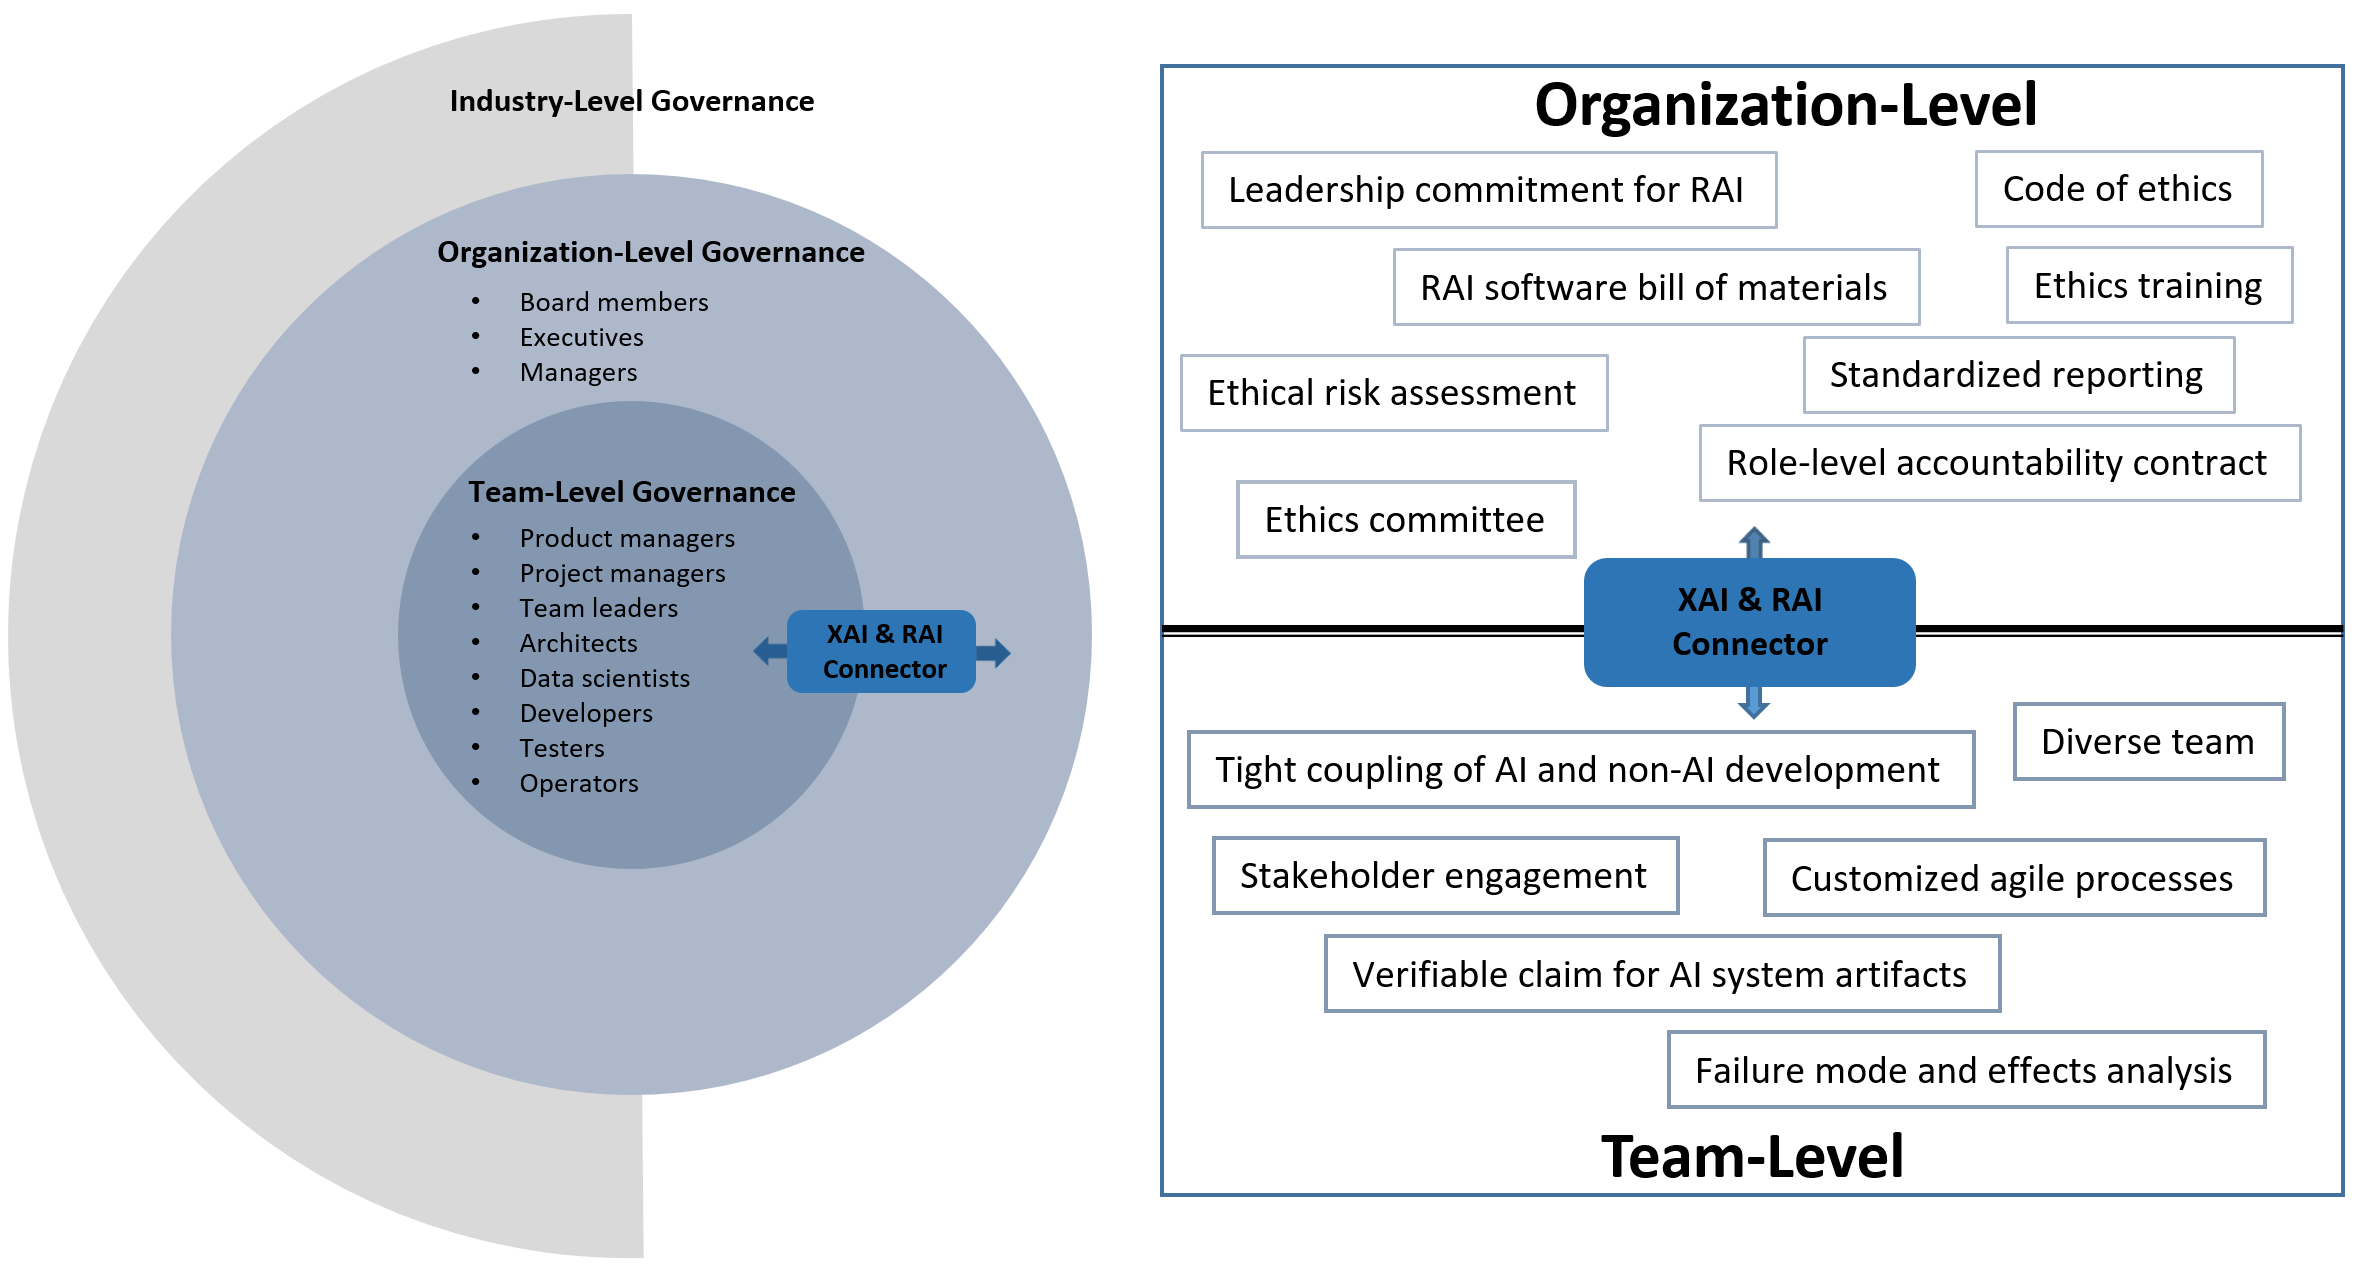
\includegraphics[width=0.8\textwidth]{Organization.png}
	\caption{A Deep Dive into the MLOps Workflow with the XRc Phase: Understanding Key Actor Roles and Responsibilities}
	\label{XAIRAIorg}
\end{figure*}
In this paper, we take a different approach by focusing on the organization-level patterns at the system level rather than just the ethical principles or AI algorithms. This approach aims to integrate responsible design in organizations into final AI products by looking at the bigger picture and the design patterns that shape the system as a whole. This is done with the intention of bridging the gap between the organizational-level and team-level and facilitating navigation. We start off by looking at the main two levels of an organization with the addition to the team-level and examine the current available methods \cite{Shneiderman, ShneidermanRespo, Jana, Hussain, roadmap}. Then we make the links on where those methods meets and create the best practices using the MLG patterns at the organization level. The overarching research question that has guided this study is:

% \begin{figure*}[h!]
% 	\centering
% 	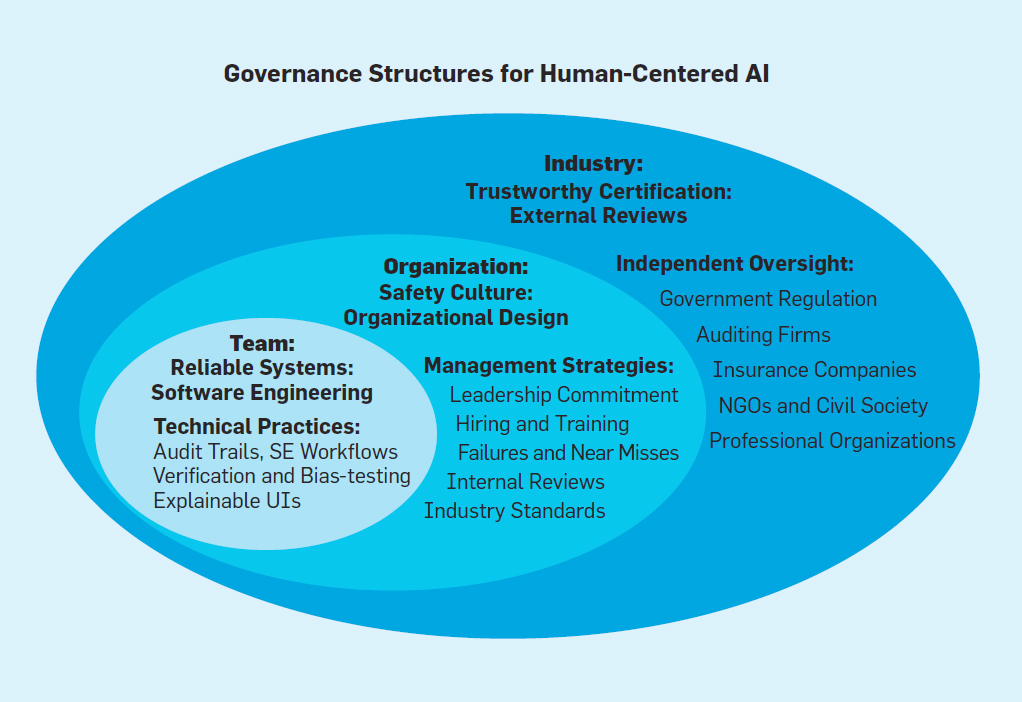
\includegraphics[width=4.74in]{governance.jpeg}
% 	\caption{Transition from traditional to the current approach}
% 	\label{ReMixMatch}
% \end{figure*}

\vskip 0.1in
\vskip 0.1in

\noindent\fbox{%
    \parbox{.48\textwidth}{%
     What is the multi-level governance pattern principle-to-practice proposed for responsible AI systems to bridge the gap between team-level and organization-level?}%
}

\vskip 0.1in
\vskip 0.1in

The main contributions of this paper are as follows:
\begin{itemize}
\item Find the link between team-level governance patterns with the organization-level patterns.
\item Suggest navigation and utilisation team-level governance patterns with the organization-level patterns.
\item Explore a case study that suits this principle-to-practice multi-level governance pattern.
\end{itemize}
\smallskip

\section{Related Work}
The issue of creating AI that is ethically accountable has garnered a great deal of interest among both industrial and academic communities. To promote ethical AI practices, a multitude of AI ethics principles and guidelines numbering around 100 have been established by various entities including governments, companies, and organizations \cite{GlobalLandscape}. However, these guidelines are often too general and theoretical for individuals involved in the implementation of AI systems to apply in real-world scenarios.

There has been a concerted effort in the field of AI to address the challenges of RAI. One approach that has gained traction is the development of algorithm-level solutions. These solutions are designed to address specific aspects of the numerous high-level AI ethics principles and guidelines that have been established by various entities. By focusing on a subset of the principles, these algorithmic solutions aim to bring concrete and practical approaches to address some of the ethical concerns related to AI. One approach that developers used is by limiting user access and preventing reverse engineering or modifications to the system design. Rather than providing full access to AI systems by running them locally, it is recommended to offer AI services through cloud-based platforms and manage interactions through APIs \cite{TobyAPI}. As an illustration, access to OpenAI's language model GPT-3 is limited to approved users who can only integrate it into their AI systems via API. Another example is Google Vision AI's facial recognition feature, which is limited to a select few celebrities and is only accessible through API. Despite these efforts, there have been instances where the algorithm has been exposed to the outside without proper internal review and verification, leading to potential issues with the responsible use of AI.

However, it's important to note that these algorithm-level solutions are just one part of the larger picture of RAI. Implementing them alone may not be enough to address all the ethical concerns related to AI, as the principles themselves are often complex and multifaceted. It requires a collaborative effort between researchers, developers, policymakers, and other stakeholders (board members, executives, managers) to ensure that AI is developed and used in an ethical and responsible manner.
\section{Methodology}
In order to build up the links of the MLG for RAI systems within organizations, we first evaluated the available methods at the team and organizational level \cite{catalogue} to understand their strengths and limitations, and identified gaps that provided opportunities for improvement. As shown in Figure \ref{XAIRAIorg}, the hierarchy of organization and team-level stakeholders in the industry is depicted on the left side of the illustration, providing a visual representation of the various levels of responsibility and decision making within the industry. The right side of the figure displays the current methods available, which are being utilized to support the operations and processes of the stakeholders.

The illustration provides a comprehensive overview of the stakeholders involved and the methods being utilized, offering insight into the strengths and limitations of the current methods. In addition, the use of XAI and RAI connectors, as shown in the illustration, can further optimize the operation of the current methods and support the efforts of the stakeholders. Utilizing these connectors can provide a more comprehensive and user-friendly experience, leading to improved outcomes and increased success for the organization and its teams.

Futhermore, we evaluated an examination of Machine Learning Operations (MLOps) technologies and tools for each stage of the project pipeline, as well as the roles involved \cite{mlops-without}. In this examination, we identified the weakness of the method being used as the absence of XAI and RAI. The lack of XAI and RAI in the method being used can result in unintended consequences and decreased trust in the system. Therefore, it is important to consider incorporating these elements into any machine learning project to ensure accountability and transparency. To best to our knowledge there is no standard for implementing the MLG pattern for RAI with XAI in MLOps.

XAI and RAI connector (XRc) can play a crucial role in connecting team-level governance to organization-level governance implementation in MLOps. By providing clear and understandable explanations for the decisions made by machine learning models, XAI helps to increase transparency and accountability at the team level. This can be especially important in complex projects involving multiple stakeholders and team members. RAI, on the other hand, helps to ensure that ethical and moral considerations are taken into account throughout the entire MLOps pipeline. This can involve creating policies and guidelines for RAI, as well as conducting risk assessments and impact evaluations. By incorporating RAI into MLOps, organizations can ensure that their use of AI aligns with their values and meets regulatory requirements.

By introducing XRc into the MLOps, organizations can bridge the gap between team-level governance and organization-level governance implementation in MLOps. This helps to ensure that AI systems are used in a responsible and ethical manner, while also providing a clear and transparent explanation of their decision-making process.

\section{Background on MLOps Workflow Stages}
Constructing a machine learning pipeline can be a challenging endeavor. The pipeline is often constructed incrementally with the assistance of tools that have limited integration capabilities. MLOps seeks to streamline this process by automating the pipeline. It serves as a combination of machine learning, data engineering, and DevOps practices, essentially streamlining and accelerating the operationalization of an ML model (including building, testing, and releasing) by incorporating DevOps practices into the process. Determining which stage should be executed by which actor in the MLOps pipeline is not a straightforward task, and often requires multiple iterations to arrive at a suitable solution. However, through the examination of multiple studies, four major stages have been identified. Subsequently, we will outline each component in detail for that particular stage.
\paragraph{Data Management Phase} Maintaining the overall quality of project-specific data can be challenging due to restrictions posed by domain-specific limitations \cite{maydanchik2007data}. These limitations can affect the consistency of the relationships between attributes, the accuracy of historical records, and the reliability of state transitions \cite{taleb2018big}. To ensure that the data models are accurate and aligned with the goals and KPIs of the project, subject-specific experts such as domain experts play a crucial role . These experts provide the necessary problem-specific questions and objectives, as well as KPIs for the data models. Additionally, they are responsible for validating the potential data and machine learning models to ensure that they meet the requirements of the project.

In some organizations, Data Stewardship is a key entity responsible for overseeing data throughout the various stages of a project. With a focus on Data Quality Management and governance, various roles such as chief, business, and technical data stewards, as well as a data quality board, have been defined to guide the data governance framework of the organization \cite{mons2018data}. The Data Stewardship plays an important role in maintaining resulting data, particularly when planning or wrapping up a project, often through a Data Management Plan (DMP).
\paragraph{ML Preparation Phase} This set of functions in the ML preparation stage deals with classic ML preprocessing tasks. Data quality is important and ensured by various roles with the help of data engineers and stewards. Implementing the ML model requires collaboration between data scientists, domain experts, and those responsible for defining the problem within the domain \cite{treveil2020introducing}. In summary, here are the functions in the ML preparation phase:
\begin{itemize}
	\item ML Data Acquisition: The ML pipeline is fed with relevant data based on the prior declared data management plan and selection by the data engineer.
	\item Data Cleaning and Labeling: The input data is cleaned and labeled for ML operations with the help of data scientists and domain experts \cite{taleb2018big}.
	\item Data Versioning: The separation of test, training, and validation data sets is crucial for the success of ML models and is achieved through data versioning.
\end{itemize}

\begin{figure*}[h!]
	\centering
	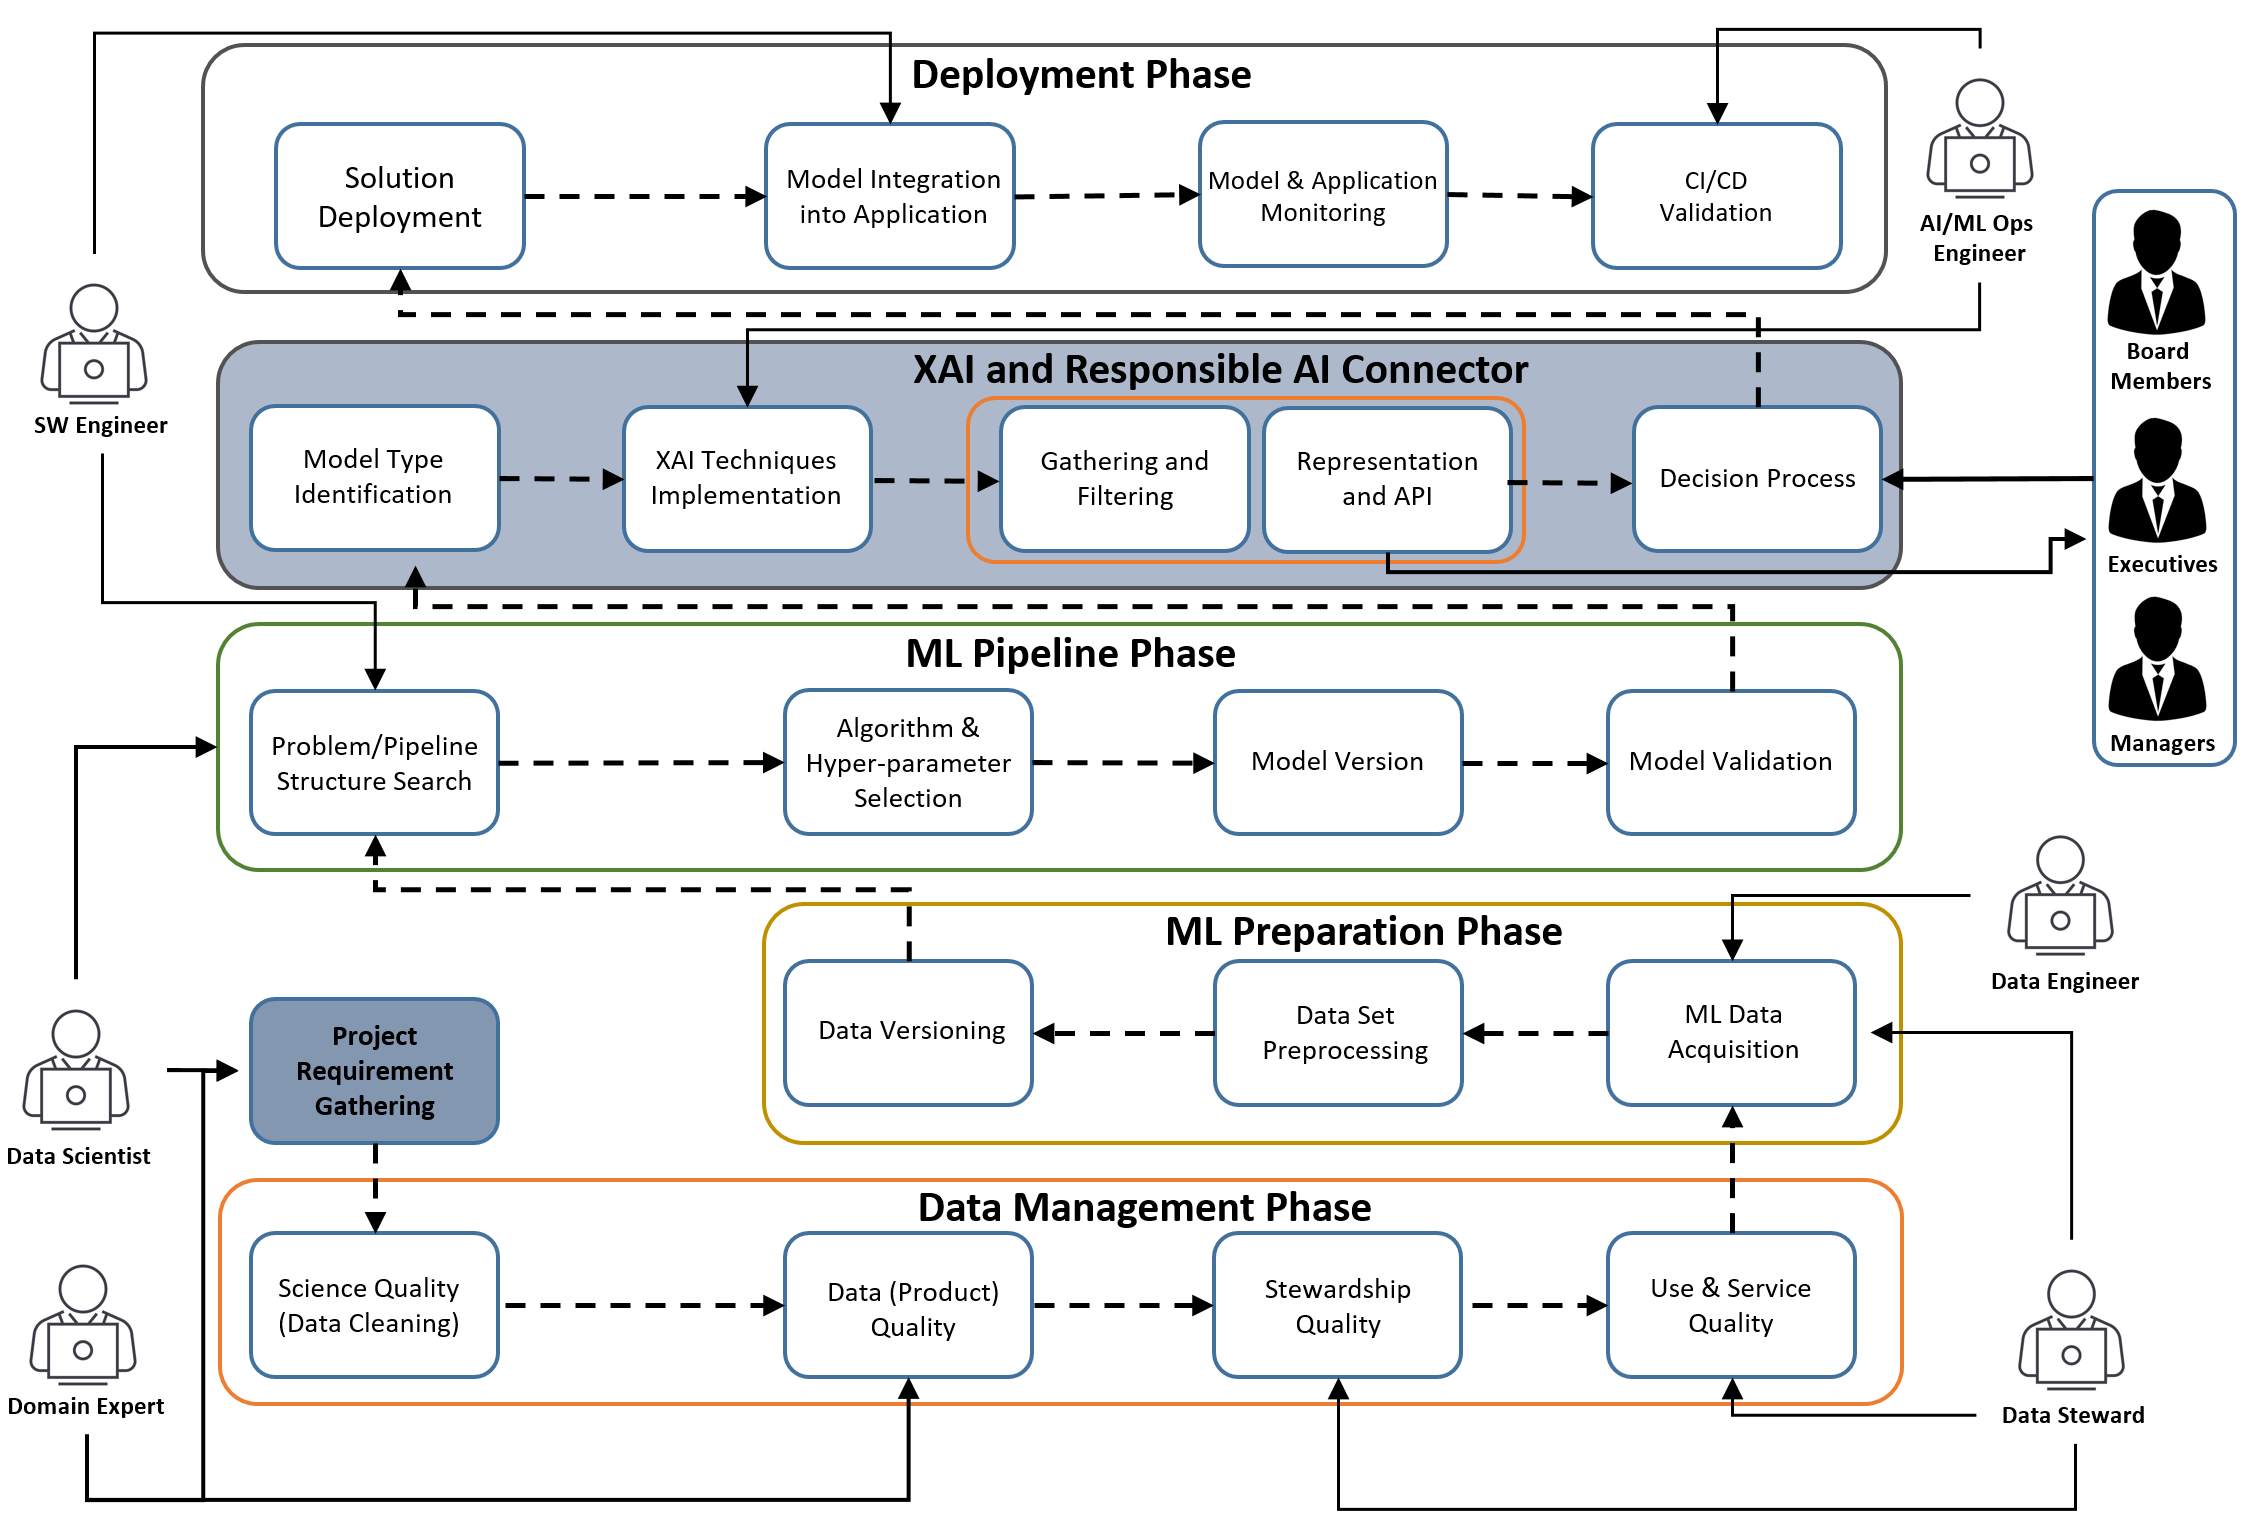
\includegraphics[width=0.8\textwidth]{ML-OPS_with_XAI.png}
	\caption{Transition from traditional to the current approach}
	\label{XRc-phase}
\end{figure*}
\paragraph{ML Training Phase}
The role of data scientists is crucial in the ML Pipeline Phase. They ensure the flexibility, scalability, and proper technology selection of the ML pipeline, while also working to improve model performance. They select the ML pipeline structure, algorithms, and hyperparameters through model versioning and validation, and are the main users in data processing for big data projects. AutoML techniques \cite{automl} and tools support data scientists and domain experts in efficiently selecting the ML pipeline and training the model. The process includes automation of feature preprocessing, model selection, and hyperparameter optimizationa. To sum up, the following functions are performed in the ML preparation phase:
\begin{itemize}
	\item Pipeline Structure Search: The structure of an ML pipeline depends on the type of data (structured or unstructured) and the technique used to solve the problem (supervised, unsupervised, or semi-supervised learning). The specific performance metrics to be used must also be defined based on the specific domain-specific requirements of the problem being solved.
	\item Algorithm and Hyperparameter Selection: The choice of the most suitable ML algorithm for a problem is made by data scientists. The algorithm's performance can be improved by adjusting its hyperparameters, such as the number of layers in a neural network \cite{kisskalt2020streamlining}. However, this process can be time-consuming and complex which addressed by AutoML in \cite{automl}.
	\item Model Versioning: It is a way to keep track of the interdependencies between an ML model, its data, framework, and modeling procedure. It is important for reverting to previous models if there is a problem in production and for deploying the correct version at the right time. Model versioning increases accountability and is an essential component for managing complex ML models.
\end{itemize}
\paragraph{Deployment Phase} The deployment stage is a pivotal moment in the MLOps process. During this phase, software engineers are responsible for incorporating the approved models into the corresponding applications and ensuring the smooth operation of the entire system. To maintain this stability, MLOps engineers must continuously monitor the model, the application as a whole, and the data being used \cite{treveil2020introducing}. Another key player in this phase is the DevOps engineer, who is in charge of constructing, testing, and deploying the functioning system. In general, it is characterized by the following tasks:
\begin{itemize}
	\item Integration of validated models into the relevant applications by software engineers.
	\item Maintenance of the operational stability of the entire system by MLOps engineers through continuous monitoring of the model, application, and data.
	\item Construction, testing, and deployment of the functioning system by DevOps engineers.
\end{itemize}

\section{XAI and RAI Connector(XRc)}
The integration of XRc into the MLOps pipeline may come with added overhead, however, it proves to be a valuable addition to the process as a whole. The addition of XRc not only reduces the risk of failure in RAI, but it also promotes efficiency by allowing for early detection of any problems with implementing organizational-level governance. This helps to avoid duplicating efforts and ensures that the RAI is being developed effectively. As shown in Figure \ref{XRc-phase}, XRc has been inserted between the ML pipeline phase and the ML deployment phase in order to analyze the changes before migrating into the application incorporating the organization level governance into the process. Let's now delve into the sub-phases of XRc.

\subsection{Model Type Identification}
Both dynamic and static identification methods can be used to identify the type of machine learning model, with dynamic methods involving examination of the model's API or performance, and static methods involving examination of the code and architecture used to implement the model.
\paragraph{Static Identification Method} In code, the type of machine learning model can be identified by examining the architecture, algorithms, and libraries used to implement the model. Understanding the architecture of the model, such as the number of hidden layers or the presence of decision trees, can give a good indication of the type of machine learning model used. Additionally, many machine learning libraries provide pre-built models with clear documentation that specify the type of model being used. The documentation for these libraries usually clearly states the type of model being used. 
For example, in the scikit-learn library \cite{pedregosa2011scikit}, the use of `LogisticRegression` class for logistic regression, which is a supervised learning algorithm, or the `KMeans` class for k-means clustering, which is an unsupervised learning algorithm.
\paragraph{Dynamic Identification Method}There are two main ways to dynamically detect the type of machine learning model:

\begin{itemize}
	\item Examining the model's API or functions: This involves looking at the functions that the model exposes, such as the `predict` function, and determining the type of model based on the inputs and outputs of the function.

	\item Examining the model's performance: This involves evaluating the model's performance on a known dataset and determining the type of model based on the performance metrics and results obtained.
\end{itemize}

The two dynamic methods can be useful in different scenarios, and the choice of method will depend on the specific requirements of the use case. For example, if the access to the model's API or functions is given, examining the API or functions might be the easiest and most straightforward way to determine the type of model. If there is no access to the API or functions, evaluating the model's performance on a known dataset might be the only option available.

\subsection{XAI techniques Implementation}
XAI techniques is implemented by AI/MLOps engineers taking into consideration the ML algorithm and the different audiences. It may require a trade-off between technical detail and simplicity, transparency and fairness, and other factors.
\paragraph{Audience evaluation} While the audiences is mainly at the organization level, AI/MLOps Engineers can categories their audience into two:
\begin{itemize}
	\item End Users: It may require simple and understandable explanations of the decisions made by a machine learning model. XAI techniques designed for this audience might include rule-based systems, decision trees, or prototype-based explanations that provide examples that are representative of the decisions made by a machine learning model.
	\item Regulators: It may require explanations of the decisions made by a machine learning model to ensure that the model is fair, transparent, and in compliance with regulations and ethical standards. XAI techniques designed for this audience might include model-agnostic techniques, such as Local Interpretable Model-Agnostic Explanation (LIME) \cite{lime} or SHapley Additive
exPlanation (SHAP) \cite{shap}, that provide explanations for the predictions made by any machine learning model.
\end{itemize}
\paragraph{ML algorithm evaluation} Since some techniques can be used and integrated together, AI/MLOps engineer have to consider the broad range of XAI techniques. Those methods can be categorized into the following categories:
Model-Agnostic Techniques: Model-agnostic XAI techniques are techniques that can be applied to any machine learning model, regardless of the underlying algorithm or architecture. Examples of model-agnostic XAI techniques include LIME and SHAP.
\begin{itemize}
	\item Model-Specific Techniques: Model-specific XAI techniques are techniques that are designed specifically for a particular type of machine learning model, such as decision trees or neural networks. Examples of model-specific XAI techniques include saliency maps for neural networks and decision trees for decision trees.

	\item Post-Hoc Techniques: Post-hoc XAI techniques are techniques that are applied to a trained machine learning model after it has been trained, in order to provide explanations for its decisions and actions. Examples of post-hoc XAI techniques include LIME, SHAP, and saliency maps \cite{kadir2001saliency}.

	\item Integrative Techniques: Integrative XAI techniques are techniques that involve integrating XAI into the training process of a machine learning model, so that explanations can be generated as part of the model's normal operation.
\end{itemize}

These categories are not mutually exclusive and some XAI techniques may fall into multiple categories. The choice of XAI technique will depend on the specific requirements of the use case and the type of model being used.

\subsection{Gathering and filtering} Gathering and filtering XAI methods involves selecting a subset of XAI methods that are appropriate for a specific use case, and then integrating and combining those methods to provide a more comprehensive and effective explanation of the decisions made by a machine learning model. To effectively utilize XAI methods for a specific use case, here are the steps to gather and filter XAI methods: 
\begin{itemize}
	\item Defining the requirements: AI/MLOps engineers should start by defining the requirements based on the audience they are trying to target and the type of model being used. This will help to determine which XAI methods are most appropriate for the use case.
	\item Gather XAI methods: Next, gathering a set of XAI methods that are appropriate and generated by the XAI technique Implementation. This may require back and forth to add, remove certain XAI techniques.
	\item Filter XAI methods: Once a set of XAI methods is gathered, filter the methods based on the specific requirements to the use case. Consider factors such as the complexity of the method, the amount of computational resources required, and the amount of technical detail that is appropriate for the audience.
	\item Combine XAI methods: After filtering the XAI methods, MLOps Engineers might consider combining methods to provide a more comprehensive and effective explanation of the decisions made by the machine learning model. They can use techniques such as multi-modal explanations, ensemble explanations, or hybrid explanations to combine XAI methods.
\end{itemize}
\begin{table*}[htbp]
\caption{Mapping of XAI Service Architecture Design to XRc MLOps Phase}
\begin{center}
\label{Mapping}
\begin{tabular}{|l|l|l|}
\hline
 & & \\
\textbf{XAI Microservices \& Provenance Ref} & \textbf{Components of XAI Microservices}  & \textbf{XRc Sub-phase Mapping} \\
 & & \\ \hline
\multirow{3}{*}{User Interface} & RESTful API & \multirow{3}{*}{Representation and API} \\
 & Web Portal & \\
 & Command Line & \\ \hline 
\multirow{4}{*}{Coordination Center} & \multirow{2}{*}{Microservice Management} & \multirow{4}{*}{Gathering and Filtering} \\
 & & \\
 & \multirow{2}{*}{XAI Operation Management} & \\
 & & \\ \hline 
\multirow{5}{*}{Microservice Layer} & Data Representation & \multirow{5}{*}{XAI Techniques Implementation} \\
 & Data Processing & \\
 & AI Model & \\
 & XAI Method & \\
 & Evaluation Metric & \\ \hline
\multirow{4}{*}{Data Persistent Layer} & Model Explanation Result & \multirow{2}{*}{XAI Techniques Implementation} \\
 & XAI Evaluation Result & \\ \cline{2-3} 
 & Machine Learning Data & \multirow{2}{*}{Model Type Identification} \\
 & Provenance Data & \\ \hline
\end{tabular}
\end{center}
\end{table*}
\subsection{Representation and API}
XAI representation refers to the format in which the explanations generated by XAI techniques are presented to the user. The representation can be in the form of text, visualizations, or other forms of data, and it depends on the specific requirements of the use case and the target audience.

An XAI API, or Application Programming Interface, is a set of protocols and tools for building software applications that provide access to XAI capabilities. An XAI API allows developers to easily integrate XAI techniques into their applications and provide explanations for the decisions made by machine learning models. For example, an XAI API might provide a set of functions that allow developers to generate explanations for specific predictions made by a machine learning model, or to visualize the model's decision-making process. The XAI API might also provide a set of data structures and protocols for representing the explanations generated by XAI techniques, such as text, visualizations, or other forms of data. Here are some ways to make the XAI API interactive:
\begin{itemize}
	\item Visualizations: Use interactive visualizations, such as heatmaps, bar charts, and scatter plots, to help stakeholders understand the explanations generated by the XAI API. This can include interactive visualizations of the model's behavior, such as feature importance, or visualizations of individual predictions, such as decision trees.
	\item User Input: Allow stakeholders to provide input to the XAI API, such as selecting specific predictions to explain, or adjusting parameters of the explanations. This can help stakeholders to better understand the explanations generated by the API, and to tailor the explanations to their specific needs.
	\item Dynamic Explanations: Provide dynamic explanations that change based on user input or other factors, such as the type of model being used, or the specific prediction being explained. This can help stakeholders to better understand the explanations generated by the API, and to see how changes in the model or input data affect the explanations.
	\item Feedback Mechanisms: Provide feedback mechanisms that allow stakeholders to provide feedback on the explanations generated by the XAI API. This can include simple feedback forms, or more complex mechanisms, such as a feedback rating system. This can help organizations to improve the quality of the explanations generated by the API, and to better meet the needs of stakeholders.
\end{itemize}

In a nutshell, XAI representation refers to the format in which XAI explanations are presented to the user, while an XAI API provides a set of protocols and tools for integrating XAI techniques into software applications and providing explanations for the decisions made by machine learning models. The choice of XAI representation and API will depend on the specific requirements of the use case and the target audience.
\subsection{Decision Process}
Incorporating an XAI API into the decision-making process at the organizational level can help stakeholders make informed decisions about whether to proceed with or stop a ML algorithm baed on the transparency and fairness of the model. To make the XAI API interactive, SW Engineers and MLOps can add features that allow stakeholders to interact with the explanations generated by the API.
\section{Case Study: Flexible XAI Service for Cloud AI Feature Contributions}
Since the XRc invoked in MLOps can target many different MLOps pipelines and cannot be easily specified, it is essential to present a specific case study to demonstrate the usability of these techniques in MLOps. In this section, we will elaborate on the Flexible XAI Service for Cloud AI Feature case study that will pick one MLOps pipeline and show the effectiveness of XRc techniques in improving its transparency and fairness.
\begin{figure*}[htbp!!]
	\centering
	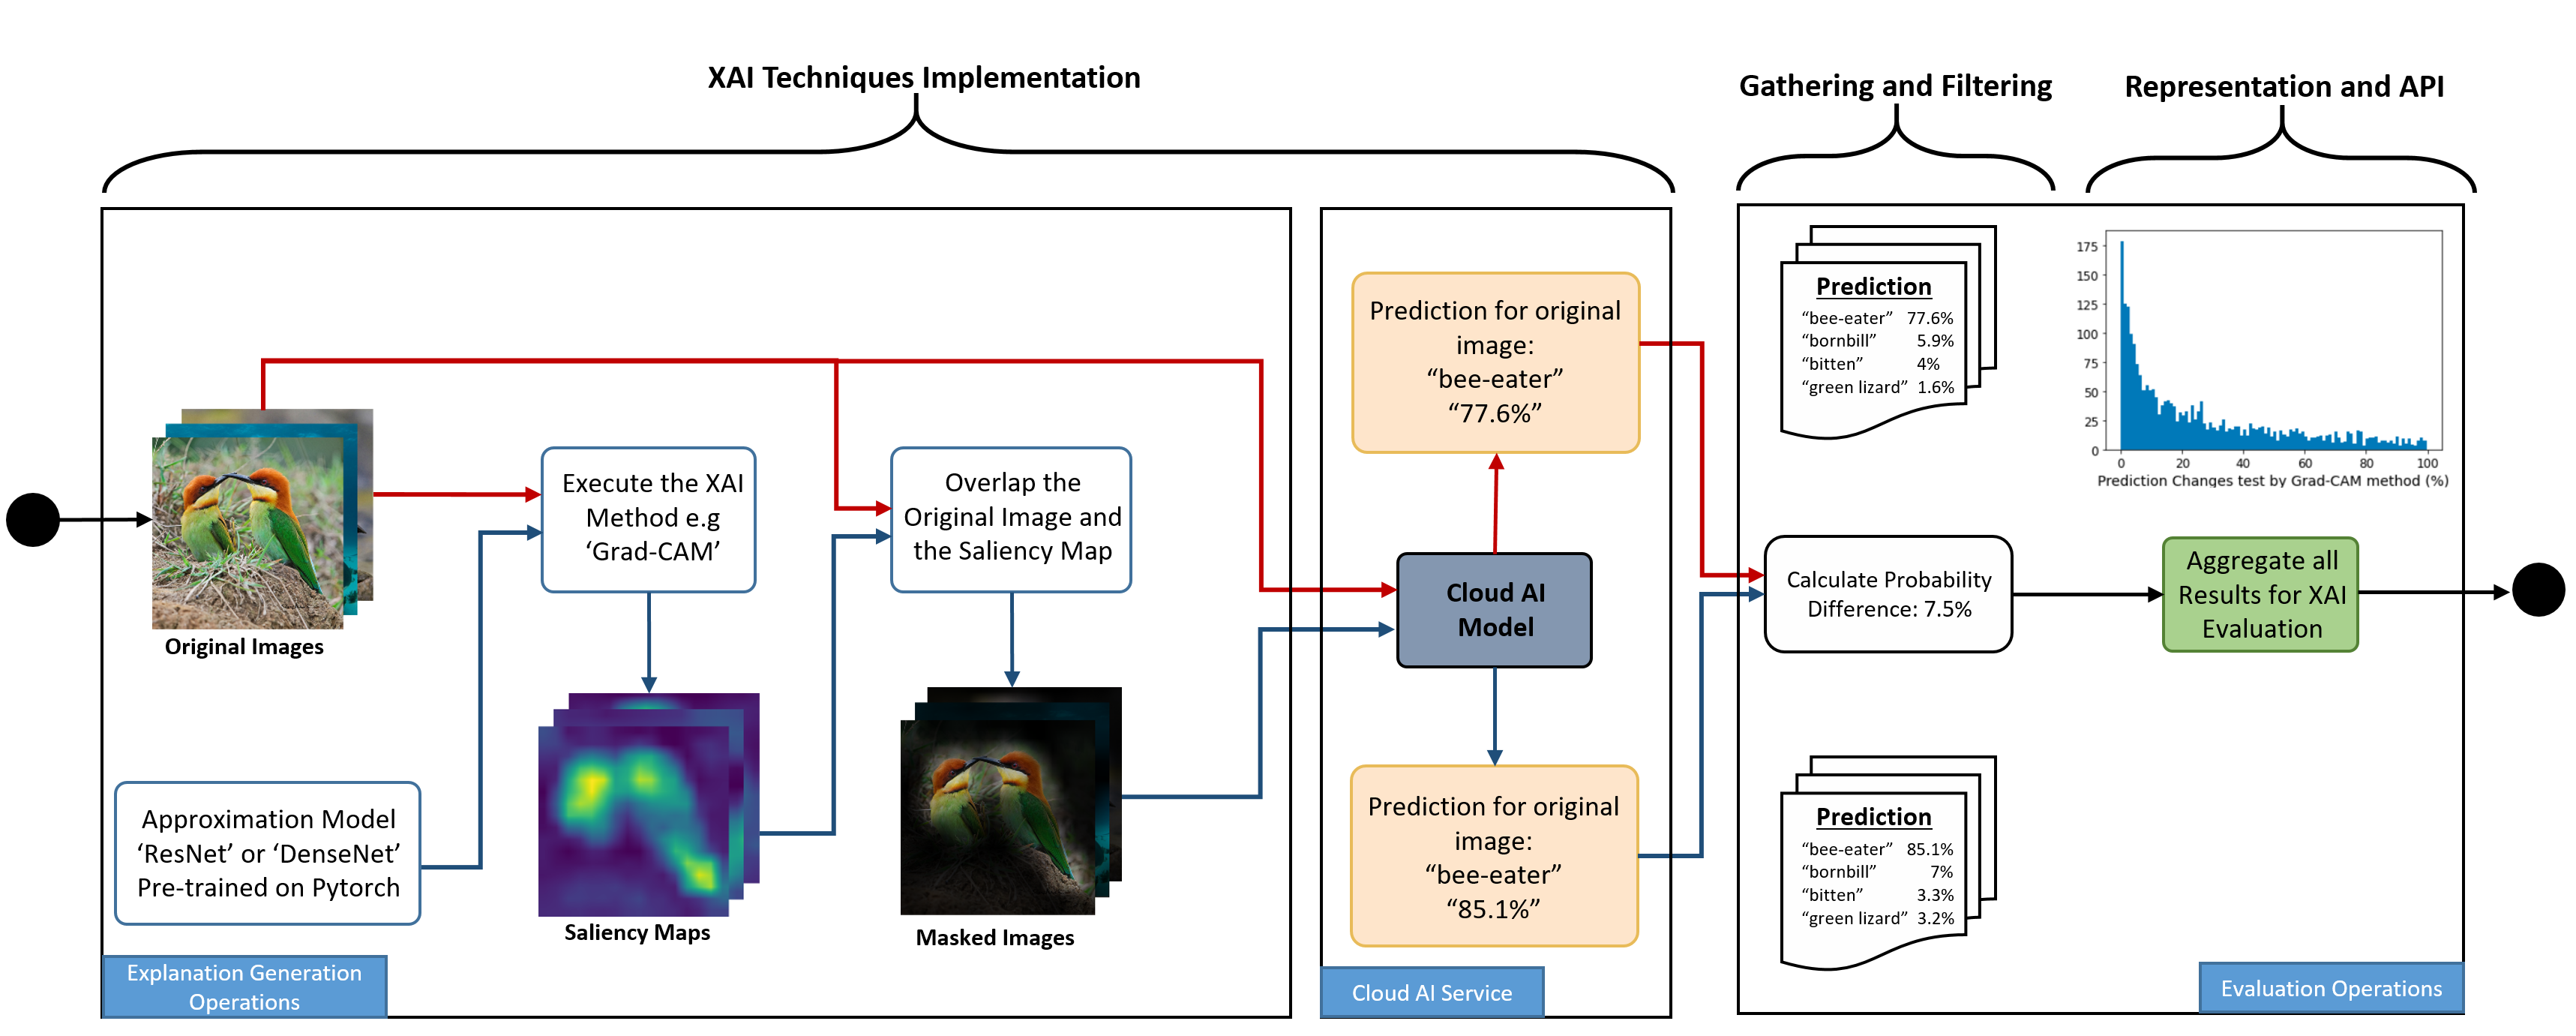
\includegraphics[width=0.9\textwidth]{XAI_MT.png}
	\caption{Mapping the Illustrated Integration of Cutting-Edge Cloud AI Services, State-of-the-Art Deep Learning Models, and Post Hoc Explainability Methods in the XRc Phase of MLOps.}
	\label{MIICE}
\end{figure*}

It is important to note that this case study will focus solely on the implementation, gathering and filtering, and representation and API \cite{TobyAPI} aspects of XRc phase in MLOps pipeline. While there are other components within the XRc phase, these sub-phases are considered to be the most critical elements within the XRc phase.

\subsection{Mapping XAI Service Architecture Design and XRc MLOps phase}
As depicted, the development of XAI operations as microservices resulted in a reference architecture composed of four layers: the user interface layer, the coordination center layer, the core microservice layer, and the data persistence layer. This reference architecture can be mapped to the XRc phase, as shown in Table \ref{Mapping}.
\paragraph{User Interface} The XAI service architecture has a user interface that allows users to set up XAI tasks or connect them to pipelines. The interface offers three forms of access: a web portal, RESTful APIs, and a command line. The web portal includes features such as task configuration, explanation summaries, and data visualization. RESTful APIs support developers in building new XAI services and executing pipelines. The command line interface allows direct communication with the back-end server. These features support the Representation and API aspect of MLOps.
\paragraph{Coordination Center} The coordination center in the XAI service architecture plays a crucial role in Gathering and Filtering in XRc Phase in the MLOps. The microservice management function is responsible for managing the life cycle of each microservice and documenting their endpoints and functional types. The XAI operation management includes a task executor that executes XAI tasks based on task sheets that contain information about the involved services, data set, and task parameters \cite{makinen}. This information is gathered and filtered by the coordination center to ensure that the correct microservices are utilized for each task. The data representation component retrieves information from the data persistence layer and presents it to the user, further supporting the Gathering and Filtering aspect of XRc Phase in MLOps.
\paragraph{Microservice Layer} The encapsulation of diverse data sets, AI models, XAI methods, and evaluation metrics into microservices as described in the previous paragraph is a key aspect of the XAI Techniques Implementation subphase of the XRc phase in MLOps. The use of microservices simplifies the integration of these entities and supports the efficient execution of XAI tasks within the MLOps pipeline. The Data Processing, AI Model, XAI Method, and Evaluation microservices each play a specific role in supporting the implementation of XAI techniques in the XRc phase, making them crucial components of the XAI Techniques Implementation subphase of the overall MLOps process.
\paragraph{Data Persistent Layer} The data persistence layer in the XAI service is responsible for managing the storage and retrieval of data sets, XAI operation data, explanation summaries, and evaluation results. This layer plays a crucial role in the XRc phase of MLOps by providing a unified system for storing and accessing the necessary information for XAI operations. The design of XAI provenance metadata is also introduced in a later section, further enhancing the efficiency and organization of the XAI process. The data persistence layer is a key component of both the XAI Techniques Implementation and Model Type Identification subphases of the XRc phase in MLOps. The ability to easily add new AI models, data sets, or XAI methods further underscores the importance of the data persistence layer in supporting the overall MLOps process.
In the next section, we will delve deeper into the implementation of the Post Hoc XAI with feature contribution explanation, highlighting its practical applications and benefits in the XRc Phase of MLOps.
\subsection{Post Hoc XAI Methods with Feature Contribution Explanation}
Post-hoc XAI methods for feature influence and causality can be applied to computer vision AI services as they provide a way to understand how the deep learning models make their predictions. These methods can be used to approximate the internal workings of the AI models and provide insights into the contribution of each feature to the prediction result. This information can be useful for improving the accuracy of the models, as well as for building trust with users and stakeholders who may be concerned about the transparency of AI systems. Additionally, the availability of state-of-the-art deep learning models and XAI methods for computer vision in the literature makes it easier to adopt these methods for computer vision AI services. 

As depicted in Figure \ref{MIICE}, the Explanation Generation Operation and the Cloud AI Service are a part of the XAI Techniques Implementation. This makes sense since the process involves inputting images into a cloud-based AI service in the first branch, which outputs the prediction results. In the second branch, the images are processed by an approximation model such as ResNet or DenseNet [35], [36]. XAI methods specific to the model [17]–[21] are then utilized to generate a salience map that highlights the most significant features of the image. This map is applied to the original image, creating augmented images that are then input into the cloud-based AI service. As a result, the prediction results from the cloud-based AI service on these augmented images will differ from the original prediction due to the changes in the features.

\section{Conclusion}
The connection between team-level governance patterns and organization-level patterns can be effectively established through the use of MLOps. The XRc phase provides a clear connection between the two levels of governance, allowing for the navigation and utilization of both patterns. The Design Explanation Microservices and Provenance case study serves as a practical example of this principle-to-practice multi-level governance pattern, showcasing how XAI techniques can be effectively implemented in real-world scenarios to support both team and organizational governance goals. By utilizing the XRc phase in MLOps and examining the results of the case study, organizations can gain a better understanding of how to bridge the gap between team-level and organizational-level governance in a way that is both effective and efficient.

Future work in this area could involve exploring new and innovative XAI techniques and methods to further enhance the efficiency and effectiveness of the XRc phase in MLOps. Additionally, continued research into the relationship between team-level and organization-level governance patterns in the context of MLOps will be important in order to fully understand the best practices and strategies for bridging the gap between these two levels of governance.
\section*{Acknowledgment}
The authors would like to extend their sincere gratitude to Zerui Wang and Jun Huang for their invaluable contributions to the case study presented in this paper. The authors acknowledge the effort and dedication of both contributors, who have made a significant impact on the outcome of this research.

\bibliographystyle{IEEEtran}
\bibliography{bibfile.bib}

\end{document}
